% (The MIT License)
%
% Copyright (c) 2023 Yegor Bugayenko
%
% Permission is hereby granted, free of charge, to any person obtaining a copy
% of this software and associated documentation files (the 'Software'), to deal
% in the Software without restriction, including without limitation the rights
% to use, copy, modify, merge, publish, distribute, sublicense, and/or sell
% copies of the Software, and to permit persons to whom the Software is
% furnished to do so, subject to the following conditions:
%
% The above copyright notice and this permission notice shall be included in all
% copies or substantial portions of the Software.
%
% THE SOFTWARE IS PROVIDED 'AS IS', WITHOUT WARRANTY OF ANY KIND, EXPRESS OR
% IMPLIED, INCLUDING BUT NOT LIMITED TO THE WARRANTIES OF MERCHANTABILITY,
% FITNESS FOR A PARTICULAR PURPOSE AND NONINFRINGEMENT. IN NO EVENT SHALL THE
% AUTHORS OR COPYRIGHT HOLDERS BE LIABLE FOR ANY CLAIM, DAMAGES OR OTHER
% LIABILITY, WHETHER IN AN ACTION OF CONTRACT, TORT OR OTHERWISE, ARISING FROM,
% OUT OF OR IN CONNECTION WITH THE SOFTWARE OR THE USE OR OTHER DEALINGS IN THE
% SOFTWARE.

\documentclass{article}
\usepackage{../pmba}
\newcommand*\thetitle{Scope Management}
\begin{document}

\plush{\pmbaTitlePage{2}}

\plush{
\pptBanner{Management Triangle}\par
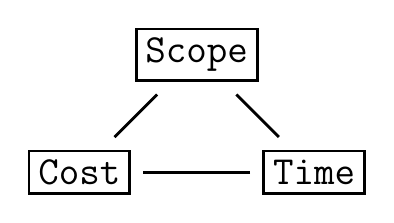
\begin{tikzpicture}[node distance=6em,
  every path/.style={draw=black, line width=.1em},
  every node/.style={font={\Large\ttfamily}, draw=black, rectangle, outer sep=.5em}]
\node (scope) {Scope};
\node[below right of=scope] (time) {Time};
\node[below left of=scope] (cost) {Cost};
\path (scope) -- (time);
\path (time) -- (cost);
\path (cost) -- (scope);
\end{tikzpicture}\par
Your responsibility, as a project manager, is to control that all three elements of the
triangle are in sync: when one of them changes you have to change the other two. If you don't
know how much the project will cost, how long will take, or how much functionality
it will implement---you are not a project manager.
}

\pmbaQuestion
  {Even though it was not required by the customer, a programmer suggests to implement an additional feature in the product, because it is obvious that users will love it; what do you say, as a PM?}
  {``Definitely, not!''}
  {``Maybe we should discuss with the customer first?''}
  {``Only if it doesn't delay all other features''}
  {``Sure, customer first!''}
  {gold-platting}

\pmbaQuestion
  {Which one is the right formulation of a functionality in a Use Case?}
  {User \emph{can} download a picture}
  {User \emph{downloads} a picture}
  {User \emph{will} download a picture}
  {User \emph{should} download a picture}
  {use-case}

\pmbaQuestion
  {A customer asks you how much work is left to be done. Where do you find this information?}
  {You ask your team}
  {Use Cases}
  {Backlog}
  {Traceability Matrix}
  {scope-control}

\pmbaQuestion
  {Which one \emph{isn't} a Non-Functional Requirement (NFR)?}
  {When ``Send'' is clicked, email must be sent in less than 500ms}
  {The ``Settings'' page must be intuitively easy to use}
  {A picture of 100Kb downloads in less than 1.5s}
  {In case of a security breach at any web server, user passwords won't leak}
  {use-case}

\pmbaQuestion
  {After six months of hard work, your team releases the product to customer's servers. The customer says: ``This is not what I wanted :('' Whose fault is it?}
  {\emph{Testers} didn't verify it earlier}
  {The \emph{customer} didn't explain what they want}
  {The \emph{project manager} didn't validate it earlier}
  {It's \emph{nobody's} fault! We don't blame! We learn and improve!}
  {V\&V}

\pmbaQuestion
  {A project of \emph{one year} and \emph{five programmers} can be decomposed into how many Work Packages?}
  {I don't know}
  {Seven}
  {25 sprints, 5 coders, 1 WPs per week \(\to\) 250 WPs}
  {Hundreds}
  {use-case}

\pmbaQuestion
  {Which estimate of project scope is the most reasonable?}
  {300,000 \emph{Hits of Code} in the repository}
  {100 \emph{Function Points} implemented}
  {500 \emph{Pull Requests} merged}
  {50,000 \emph{Lines of Code} written}
  {estimate}

\plush{
  \pptBanner{Read this:}

  \href{https://www.youtube.com/watch?v=RglMmJb0PZ4}{SSD 2/16: Lecture about Requirements Engineering} (2022)

  Wikipedia:
  \href{https://en.wikipedia.org/wiki/COSMIC_functional_size_measurement}{COSMIC},
  \href{https://en.wikipedia.org/wiki/Function_point}{Function Point},
  \href{https://en.wikipedia.org/wiki/MoSCoW_method}{MoSCoW method}

  \nospell{Karl Wiegers} et al., \emph{Software Requirements} (1999)

  \nospell{Alistair Cockburn}, \emph{Writing Effective Use Cases} (1999)

  \href{https://www.yegor256.com/2014/04/26/incremental-requirements-with-requs.html}{Incremental Requirements With Requs} (2014)

  \href{https://www.yegor256.com/2015/11/10/ten-mistakes-in-specs.html}{10 Typical Mistakes in Specs} (2015)

  \href{https://www.yegor256.com/2014/10/20/how-we-write-product-vision.html}{How We Write a Product Vision} (2014)
}

\end{document}
